% ---------------------------------------------------------------------
% ---------------------------------------------------------------------
% ---------------------------------------------------------------------

\chapter[Multiway data, methods for its analysis]{Multiway data, methods for its analysis}



% ---------------------------------------------------------------------
% ---------------------------------------------------------------------
\section{From 2D matrices to 3D arrays}
In most fields, data sets are usually represented by two dimensional matrices, where the rows are the observations and the columns are the different variables ($I \times J$). But in metabolomics, and in general in many other omic sciences, sometimes these $I \times J$ data sets can be expanded by taking for example, repeated measurements at different $K$ time points for each observation and producing a three-dimensional data structure ($I \times J \times K$) called three-way array (\autoref{figura27}) or, more generally, a multidimensional data structure called multi-way array. Most of the modelling methods that have been explained in \autoref{chapter:modern_techniques} are not able of dealing with such data structures, which raise many methodological complications to the analyses. Therefore, different three-way or multi-way specific methods have been developed during the last decades to deal with this sort of data.

\begin{figure}[hbtp]
\centering
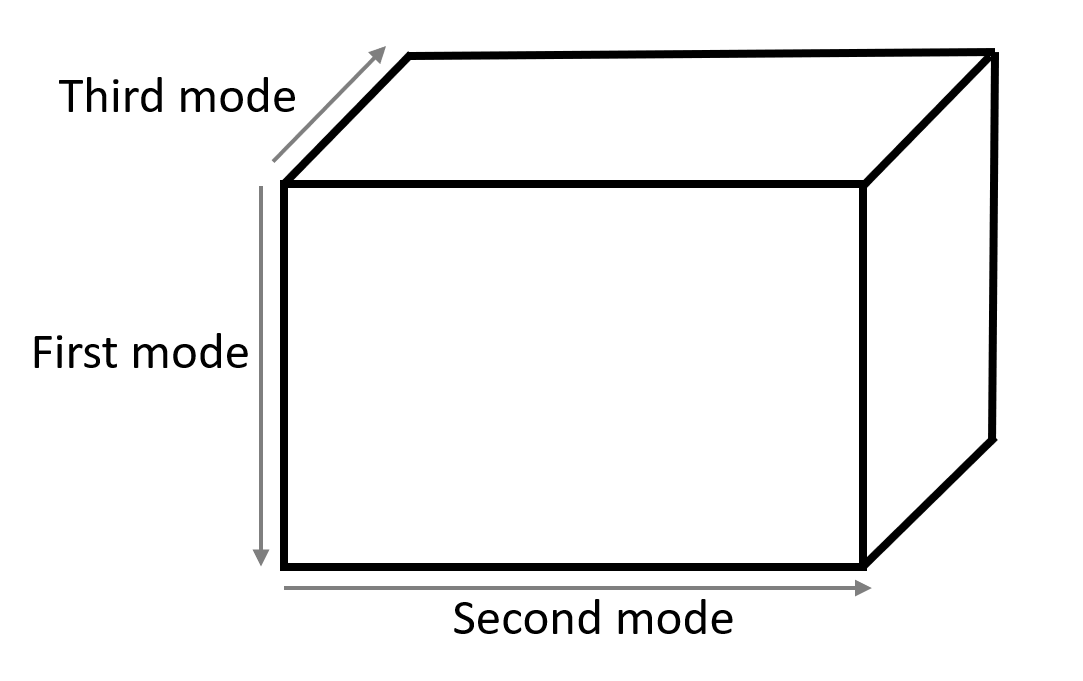
\includegraphics[width=0.65\textwidth]{figura27.png}
\caption{Representation of a three-way array.}
\label{figura27}
\end{figure}

\section{Exploration of N-way arrays}
\subsection{Tucker3}
When studying multi-way structures, the most general model that can be used is the Tucker3 model \parencite{tucker1966some}, also explained in detail by \cite{kiers2001three}.

\section{Regression methods for N-way arrays, N-PLS}
\label{NPLSregression}
N-PLS studies relationships between some three-way (or N-way) \textbf{\underline{X}} (e.g. I x J x K) data structure and any \textbf{\underline{Y}} (e.g. I x L x M) data structure. It is the natural extension of PLS to \textit{N}-way structures, which tries to maximize the covariance between \textbf{\underline{X}} and \textbf{\underline{Y}} data arrays. Considering \textbf{X} (IxJK) the unfolded version of \textbf{\underline{X}}, \textit{N}-PLS tries to find latent spaces $\textbf{\text{W}}^{J}$ and $\textbf{\text{W}}^{K}$ that maximize the covariance between \textbf{X} and \textbf{Y}, so it can be expressed as:

\begin{equation}
\textbf{\text{X}}=\textbf{\text{T}}(\textbf{\text{W}}^{K}|\otimes{}|\textbf{\text{W}}^{J})^{T}+\textbf{\text{R}}
\label{equation01}
\end{equation}

Afterwards decomposing \textbf{\underline{X}} from \textbf{X} using the improved $N$-PLS version expression \parencite{bro2001difference}, in order to obtain residuals with better statistical properties:

\begin{equation}
\textbf{\text{X}}=\textbf{\text{T}}\textbf{\text{Gu}}(\textbf{\text{W}}^{K}\otimes{}\textbf{\text{W}}^{J})^{T}+\textbf{\text{R}}^{\boldsymbol{\prime{}}}
\label{equation02}
\end{equation}

In the same way, \textbf{\underline{Y}} can be decomposed by unfolding \textbf{\underline{Y}} ($I \times L \times M$) into \textbf{Y} ($I \times LM$) as:

\begin{equation}
\textbf{\text{Y}}=\textbf{\text{U}}(\textbf{\text{Q}}^{M}|\otimes{}|\textbf{\text{Q}}^{L})^{T}+\textbf{\text{R}}^{\boldsymbol{\prime{}\prime{}}}
\label{equation03}
\end{equation}

In this case, $\textbf{\text{W}}^{K}$ and $\textbf{\text{W}}^{J}$ refer to the weights of the third and of the second mode, respectively; whereas $\textbf{\text{T}}$ matrix gathers the scores of the samples at each component extracted, in the first mode. $|\otimes{}|$ is the Khatri-Rao product and $\otimes{}$ the Kronecker product, which forbid or allow (respectively) to take interactions between the different modes components into account. 
\textbf{Gu} is the core array (unfolded) of a Tucker3 decomposition when using \textbf{T}, $\textbf{\text{W}}^{K}$ and $\textbf{\text{W}}^{J}$ as loadings, in order to obtain a better (or at least not worse) approximation of the \textbf{\underline{X}} array \parencite{smilde2005multi}. Finally, $\textbf{\text{R}}^{\boldsymbol{\prime{}}}$ incorporates the residuals. Analogously, \textbf{U} refers to the \textbf{Y} scores, and $\textbf{\text{Q}}^{M}$ and $\textbf{\text{Q}}^{L}$ to the loadings of the array \textbf{\underline{Y}}.
Finally, from the scores \textbf{T} and \textbf{U}, as well from the \textbf{W} weights, a $\textbf{\text{B}}_{PLS}$ regression matrix can be obtained \parencite{bro1998multi} so

\begin{equation}
\textbf{\text{Y}}=\textbf{\text{X}}\textbf{\text{B}}_{PLS}+\textbf{\text{R}}^{\boldsymbol{\prime{}\prime{}\prime{}}}
\label{equation04}
\end{equation}

